% \documentclass[review]{elsarticle}
\documentclass[utf8, babel, sor, jor, amsmath, amssymb, reprint]{elsarticle} %удалить перед отправкой
\usepackage[T2A]{fontenc} %удалить перед отправкой
\usepackage[utf8x]{inputenc} %удалить перед отправкой
\usepackage[english,russian]{babel} %удалить перед отправкой
\graphicspath{{images/}}

\usepackage{lineno,hyperref}
\usepackage{algorithm}
\usepackage{algorithmic}
\modulolinenumbers[5]

\journal{Journal of \LaTeX\ Templates}

\bibliographystyle{elsarticle-num}

\usepackage{mathrsfs}
\usepackage{amsmath}
\usepackage{amssymb}%



%%%%%%%%%%%%%%%%%%%%%%%
%% Elsevier bibliography styles
%%%%%%%%%%%%%%%%%%%%%%%
%% To change the style, put a % in front of the second line of the current style and
%% remove the % from the second line of the style you would like to use.
%%%%%%%%%%%%%%%%%%%%%%%

%% Numbered
%\bibliographystyle{model1-num-names}

%% Numbered without titles
%\bibliographystyle{model1a-num-names}

%% Harvard
%\bibliographystyle{model2-names.bst}\biboptions{authoryear}

%% Vancouver numbered
%\usepackage{numcompress}\bibliographystyle{model3-num-names}

%% Vancouver name/year
%\usepackage{numcompress}\bibliographystyle{model4-names}\biboptions{authoryear}

%% APA style
%\bibliographystyle{model5-names}\biboptions{authoryear}

%% AMA style
%\usepackage{numcompress}\bibliographystyle{model6-num-names}

%% `Elsevier LaTeX' style
\bibliographystyle{elsarticle-num}
%%%%%%%%%%%%%%%%%%%%%%%


\usepackage{xcolor}
\newcommand{\todo}[1] {\textcolor{red}{#1}} %%for TODO comments
\def\l{\left\langle}
\def\r{\right\rangle}

\usepackage{mathrsfs}
\usepackage{amsmath}
\usepackage{amssymb}%


\begin{document}

\begin{frontmatter}


\title{Ground state search 2D Ising model}

\author[mainaddress, secondaryaddress]{Viacheslav Trukhin\corref{mycorrespondingauthor}}
\ead{trukhin.vo@dvfu.ru}

\author[mainaddress]{Egor Prokhorov\corref{mycorrespondingauthor}}
\ead{prokhorov.ei@dvfu.ru}

\author[mainaddress, secondaryaddress]{Konstantin Nefedev\corref{mycorrespondingauthor}}
\ead{nefedev.kv@dvfu.ru}


\address[mainaddress]{Far Eastern Federal University, Vladivostok, Russky Island, 10 Ajax Bay, 690922, the Russian Federation}
\address[secondaryaddress]{Institute of Applied Mathematics, Far Eastern Branch, Russian Academy of Science, Vladivostok, Radio 7, 690041, the Russian Federation}

\begin{abstract}


\end{abstract}


\begin{keyword}
Ising model, GPU and CPU high performance calculations, spin ice, spin glass, statistical thermodynamics.

\end{keyword}


\end{frontmatter}

\linenumbers
\newpage
\tableofcontents

\newpage
\section{Введение}

Всего несколько процентов имеющих магнитный момент атомов, случайно распределенных в немагнитном носителе, таком, например, как благородный металл  \cite{finkler1989spin}, образуют спиновое стекло \cite{belokon2006spin}, которое позволило получить множество интересных экспериментальных результатов. Эти результаты положили начало целому ряду новых тем научных исследований, в частности, в области статистической механики и физики конденсированных сред.

Модель Эдвардса-Андерсона (ЕА) спинового стекла Изинга является одним из простейших примеров моделей спиновых стекол с короткодействующими взаимодействиями. Несмотря на кажущуюся простоту, свойства этой модели для 2D и более высоких размерностей до сих пор не очень хорошо изучены, и даже многие из ее важнейших свойств при Т=0 неизвестны \cite{pal1996ground}. Свойства основного состояния модели Изинга различных решеток с конкурирующими ферромагнитными и антиферромагнитными взаимодействиями изучаются на протяжении множества лет \cite{lebrecht2004plaquette, valdes2012j, lebrecht2015j}. 

В настоящее время модель Изинга актуальна не только в области физики твердого тела, но также находит применение в нейробиологии, моделировании опухолей и описании критических газожидкостных явлений. Несмотря на многие годы интенсивных исследований, природа низкотемпературной фазы модели Изинга фрустрированных спиновых систем с ограниченным радиусом взаимодействия остается невыясненной \cite{newman2023proof}. Два наиболее важных открытых вопроса касаются свойств спиновых стекол при нулевой температуре, в частности, число основных состояний и природа низкоэнергетических возбуждений \cite{newman2022ground}.  

Расчет конфигураций основного состояния спинового стекла с заданным Гамильтонианом является одной из самых сложных оптимизационных задач. В трехмерном случае задача является $NP$-трудной \cite{barahona1982computational, hartmann2002optimization}, что означает ни один известный алгоритм не может решить задачу поиска основного состояния за время, пропорциональное степени линейного размера системы, и считается, что такой алгоритм не может быть разработан. В настоящее время алгоритма, обладающего одновременно высокой точностью и эффективностью, не существует \cite{fan2023searching}.

Изучение спиновых стекол является активной и противоречивой областью статистической физики. В частности, свойства спиновых стекол при нулевой температуре интенсивно изучаются приближенными методами \cite{perez2012ground}. В настоящее время разрабатываются различные приближенные подходы для решения моделей спиновых систем \cite{farias2024differentiable, rybin2022hybrid, makarova2023canonical}. 

Модели спиновых систем на решетках представляют собой идеальную платформу для исследования сложных магнитных основных состояний с возбуждениями, что чрезвычайно важно для физики конденсированного состояния и материаловедения \cite{lacroix2011introduction}. В т.ч. исследования критический полей переключения между основными состояниями, скачков энтропии при переключениях между основными состояниями, корреляционных функций \cite{ramirez2004effect, rosas2004random, andriushchenko2019large}. Попытки приближенного вычисления энергии основного состояния и энтропии в модели спинового стекла Эдвардса-Андерсона на плоской решетке предпринимались \cite{perez2012ground}, однако даже в приближении задача двумерной плотности низкоэнергетическом состояний является трудноразрешимой. Для некоторых решеток, например, для треугольной, все же удается получить информацию об энтропийных и магнитных свойствах \cite{jurvcivsinova2024classical}.

Исследование энергетического ландшафта низкоэнергетических состояний является актуальной задачей \cite{biswas2023energy}. Интересный вопрос касается того, при какой концентрации ферромагнитных обменных взаимодействий относительно концентрации антиферромагнитных обменных будет наблюдаться переход между состоянием (анти-)ферромагнетизма и состоянием спинового стекла \cite{zimmer2022role}. Термодинамические свойства и фазовая диаграмма основного состояния относительно небольшого числа спинов молекулярных кластеров рассчитаны в работе \cite{dias2023ground}.

Конфигурации основных состояний, а также возбуждения в основных и низкоэнергетических конфигурациях искусственного спинового льда, наряду с макроскопическим вырождением основного состояния и остаточной энтропией  при низких температурах активно исследуются в модели дальнодействующего дипольного взаимодействия \cite{makarova2021low, singh2024micromagnetic}.

Задача оценки энергии основного состояния, а также выяснение природы его макроскопического вырождения являются открытыми множество лет. При низких температурах спиновое стекло в основном состоянии проявляет свойства, которые доминируют в его температурном поведении. Пока точного решения не получено, а данные, которые приводятся в литературе, весьма противоречивы. Для $N\rightarrow \infty$ оценки энергии основного состояния различными методами Thouless-Anderson-Palmer (TAP) Approach
$E_{gs}=0$ \cite{thouless1977solution}; 
метод реплик $E_{gs}=-2/\pi$ \cite{sherrington1975solvable}; partition function $E_{gs}=-0.5$ \cite{tanaka1980analytic}; mean random field $E_{gs}=-1/\sqrt{2\pi}$ \cite{klein1976comparison}; 
Монте-Карло $E_{gs}=-0.76$ \cite{kirkpatrick1978infinite};
алгоритм Шраудольфа-Каменецкого $E_{gs}=-1.33$ \cite{karandashev2019global}; метод параллельного отжига Монте-Карло $E_{gs}=-1.40193$ \cite{palmer1999ground}; $E_{gs}=-1.40197$ \cite{campbell2004energy}; $E_{gs}=-1.4009$ \cite{roma2009ground}; метод параллельного отжига Монте-Карло  $E_{gs}=-1.31479$ \cite{roma2009ground}. 

Для конечного числа спинов, и энергия основного состояния будет зависеть очень сильно от конкретной реализации нормального распределения $\left\lbrace J_{ij} \right\rbrace $. Для оценки энергии основного состояния системы конечного числа спинов может быть использован алгоритмы, в т.ч. исчерпывающего перечисления \cite{padalko2021parallel}. В настоящей работе предлагается новый подход к вычислению основных состояний модели Эдвардса Андерсона. Мы получили соответствие решение алгоритмом декомпозиции для энергии основного состояния и остаточной энтропии с решением полученным алгоритмом исчерпывающего перечисления.  

Задачи:

1. Построить график $S(P_+)$ Остаточная энтропия $S$ в зависимости от обменной константы $P_+$ для N=10x10

2. Исследовать зависимость вырождения основного состояния от количество и распределения кластеров из плакетов. 

\section{Решение исчерпывающим перечислением}

Модель спинового стекла Эдвардса-Андерсона представляет собой плоскую решетку Изинга:

\begin{equation}
	E = -\sum J_{ij} S_i S_j,
	\label{eq:ising_energy}
\end{equation}

 где обменные интегралы $J$ могут принимать значения +1 или -1 создавая таким образом приближение аморфных материалов

Для решения такой цепочки из трёх спинов статистическая сумма
принимает вид:

\begin{equation}
	Z = e^{3\beta - 3\beta h} + 3e^{\beta - h - \beta} + 3e^{\beta h - \beta} + e^{3\beta + 3\beta h}
	\label{eq:stat_3}
\end{equation}

\section{Решение методом декомпозиции}

Рассматривая разные квадратные решётки из четырёх спинов взаимодействующих лишь с ближайшими соседями, можно заметить, что фрустрация в основном состоянии обязательно появляется, если в системе три обменных интеграла одного знака, а четвёртый другого.

\begin{figure}[h]
	\centering
	\resizebox{240px}{120px}{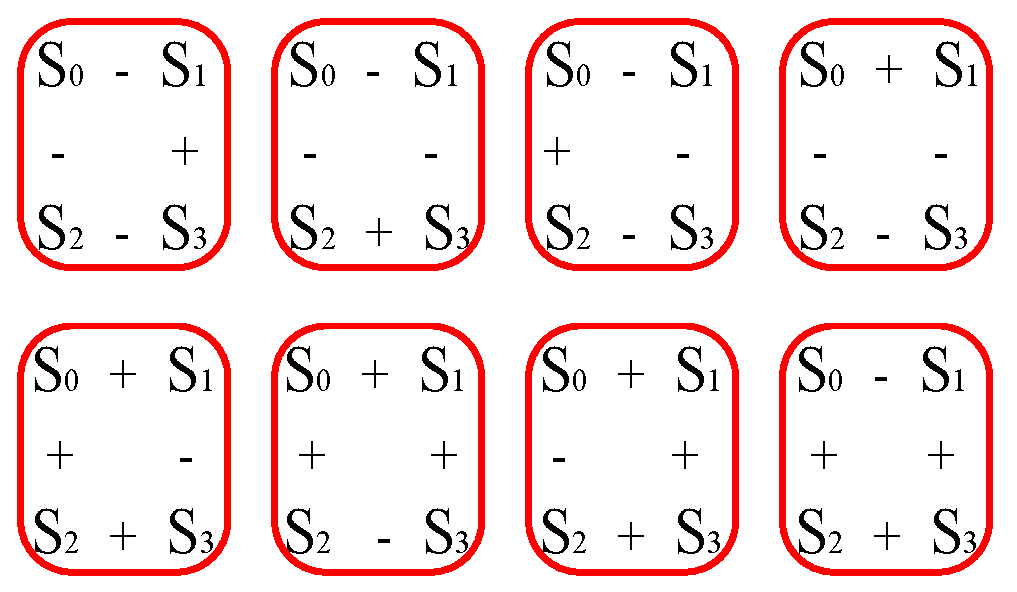
\includegraphics{2x2.1.eps}}
	\caption{Фрустрированные квадратные системы}
	\label{fig:label}
\end{figure}

Полная энергия таких систем в соответствии с формулой \eqref{eq:ising_energy} принимает вид:

\begin{equation}
	E = -J_{01} S_0 S_1-J_{02} S_0 S_2-J_{13} S_1 S_3-J_{23} S_2 S_3.
	\label{eq:ising_energy_2x2}
\end{equation}

Поиск основного состояния данных систем методом полного перебора показывает, что каждая из этих систем имеет 8 основных состояний. Таким образом в основном состоянии каждая из пар спинов может быть фрустрирована.

Тогда логично предположить, что если система состоит из двух таких подсистем, то для минимизации энергии фрустрированная пара должна быть расположена на пересечении этих подсистем.
На Рис.2 пример решётки, состоящей из двух квадратных фрустрированных подсистем. Фрустрированной парой спинов будет пара $S_1$,$S_4$.

\begin{figure}[h]
	\centering
	\resizebox{70px}{70px}{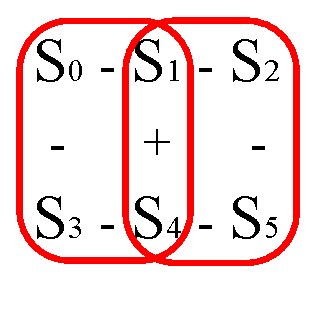
\includegraphics{3x2.eps}}
	\caption{Решётка,состоящая из двух квадратных фрустрированных подсистем}
	\label{fig:label}
\end{figure}


Метод полного перебора подтверждает правильность данного решения. В Таблице 1 приведены низкоэнергетические состояния данной решётки, полученные с помощью полного перебора состояний. Конфигурации спинов в основных состояниях доказывают что фрустрированной парой является пара $S_1$,$S_4$

\begin{table}[h]
	\centering
	\begin{tabular}{|c|c|}
		\hline
		 E   &   Фрустрированная пара \\
		 \hline
		-5   &  $S_1=1$, $S_4=-1$ \\
		\hline
		-5   &   $S_1=-1$, $S_4=1$ \\
		\hline
	\end{tabular}
	\caption{Основные состояния решётки}
	\label{tab:gs}
\end{table}

Таким образом, зная где расположена фрустрированная пара спинов, а следовательно, и где расположены не фрустрированные пары, можно найти основное состояние системы просто расставляя значение спинов по порядку или с начиная с любого спина. Полученная данным методом конфигурация и значение энергии также соответствуют основному состояния приведенном в Таблице \eqref{tab:gs}.

Примечательно, что расположение фрустрации в подобных системах не зависит от знака обменного интеграла конкретной пары. Главное чтобы сохранялось правило, что в каждой квадратной системе три обменных интеграла одного знака и один другого. 

\begin{figure}[h]
	\centering
	\resizebox{75px}{70px}{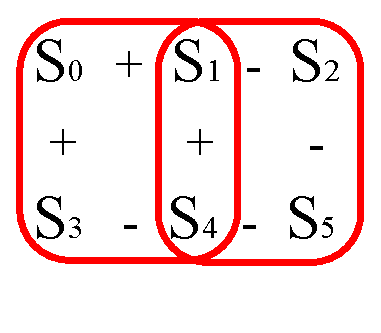
\includegraphics{3x2.2.eps}}
	\caption{Решётка, состоящая из двух квадратных фрустрированных подсистем}
	\label{fig:label2}
\end{figure}

На рисунке \eqref{fig:label2} показан пример другой решётки, состоящей из двух квадратных фрустрированных подсистем.

\begin{table}[h]
	\centering
	\begin{tabular}{|c|c|}
		\hline
		E   &   Фрустрированная пара \\
		\hline
		-5   &  $S_1=1$, $S_4=1$ \\
		\hline
		-5   &   $S_1=-1$, $S_4=-1$ \\
		\hline
	\end{tabular}
	\caption{Основные состояния решётки}
	\label{tab:gs2}
\end{table}

Несмотря на другие знаки обменных интегралов в таблице \eqref{tab:gs2} видно, что фрустрированной парой также является пара $S_1$,$S_4$.

Также стоит отметить, что на расположение фрустрации в таких рештках не влияют другие квадратные подсистемы, если они не являются фрустрированными.

\begin{figure}[h]
	\centering
	\resizebox{180px}{150px}{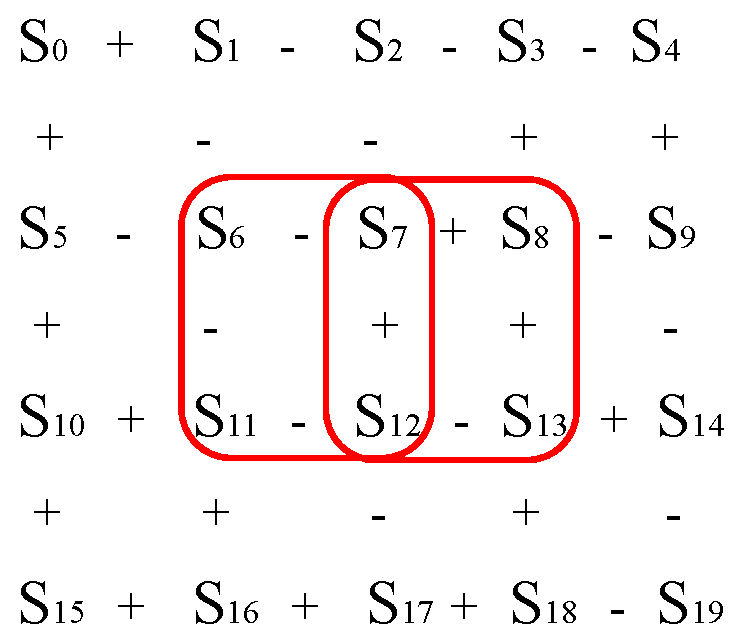
\includegraphics{5x4.eps}}
	\caption{Решётка из двадцати спинов, обладающая двумя фрустрированными подсистемами}
	\label{fig:label3}
\end{figure}

На рисунке \eqref{fig:label3} представлена система из двадцати спинов, в центре которой находятся две квадратные фрустрированные подсистемы. Исходя из предыдущих размышлений, данная система должна обладать одной фрустрированной парой  $S_7$,$S_12$.

\begin{table}[h]
	\centering
	\begin{tabular}{|c|c|}
		\hline
		E   &   Фрустрированная пара \\
		\hline
		-29   &  $S_7=1$, $S_{12}=1$ \\
		\hline
		-29   &   $S_7=-1$, $S_{12}=-1$ \\
		\hline
	\end{tabular}
	\caption{Основные состояния решётки, состоящей из 25 спинов}
	\label{tab:gs3}
\end{table}

Поиск основных состояний методом исчерпывающего перечисления подтверждает правильность рассуждений \eqref{tab:gs3}.

Если рассматриваемые квадратные фрустрированные решётки пересекаются с несколькими себе подобными, то они формируют кластер.

\begin{figure}[h]
	\centering
	\resizebox{150px}{75px}{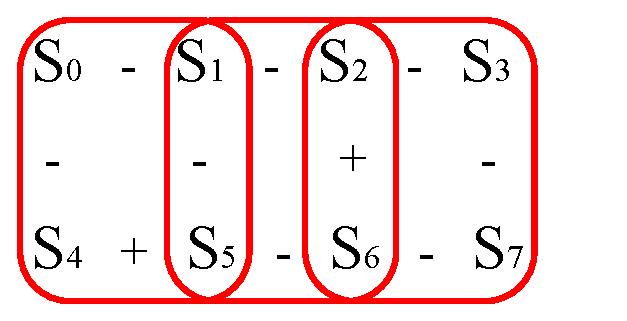
\includegraphics{4x2.eps}}
	\caption{Кластер фрустрированных квадратных решёток}
	\label{fig:cluster}
\end{figure}

В кластере необходимо выбрать фрустрированными пары, находящиеся на пересечении так чтобы такая пара была в подсистеме только одна. Если в каком-то состоянии подсистема осталась без выбранной пары в силу невозможности её расположения на пересечении подсистем, выбирается одна из трёх оставшихся в подсистеме пар, по возможности та, которая не будет возбуждать другие подсистемы, не входящие в кластер .Это можно сделать с помощью полного перебора состояний пар, где состояние пары может принимать только два значения: пара фрустрирована и пара не фрустрирована.

В данной системе \ref{fig:cluster} можно выбрать фрустрированной пару $S_1$,$S_5$, тогда пару  $S_2$,$S_6$ выбрать уже нельзя. Второй фрустрированной парой можно выбрать оду из трёх оставшихся в подсистеме пар: $S_2$ $S_3$, $S_3$,$S_7$ или $S_6$,$S_7$. Если изначально выбирается пара $S_2$ $S_6$, то второй будет пара $S_0$ $S_1$, $S_0$,$S_4$ или $S_4$,$S_5$. Далее для каждой из конфигураций фрустраций в системе расставляются значения спинов. Таким образом для данной системы получается 12 основных состояний.

Полный перебор состояний данной системы подтверждает правильность расстановки фрустраций в решётке, энергию и кратность вырождения.

\begin{table}[h]
	\centering
	\begin{tabular}{|c|c|}
		\hline
		E   &   Фрустрированная пара \\
		\hline
		-6   &  $S_1=1$, $S_5=1$\\
		      &    $S_2=-1$, $S_3=-1$ \\
		 \hline
		 -6   &  $S_1=1$, $S_5=1$\\
		      &    $S_3=1$, $S_7=1$ \\
		 \hline
		 -6   &  $S_1=1$, $S_5=1$\\
		      &    $S_6=-1$, $S_7=-1$ \\
		 \hline
		-6   &  $S_2=1$, $S_6=-1$\\
				&    $S_4=-1$, $S_5=1$ \\
		 \hline
		-6   &  $S_2=1$, $S_6=-1$\\
				&    $S_0=-1$, $S_1=-1$ \\
		 \hline
		-6   &  $S_2=1$, $S_6=-1$\\
				&    $S_0=1$, $S_4=1$ \\
		\hline
		-6   &  $S_1=-1$, $S_5=-1$\\
			&    $S_2=1$, $S_3=1$ \\
		\hline
		-6   &  $S_1=-1$, $S_5=-1$\\
			&    $S_3=-1$, $S_7=-1$ \\
		\hline
		-6   &  $S_1=-1$, $S_5=-1$\\
			&    $S_6=1$, $S_7=1$ \\
		\hline
		-6   &  $S_2=-1$, $S_6=1$\\
			&    $S_4=1$, $S_5=-1$ \\
		\hline
		-6   &  $S_2=-1$, $S_6=1$\\
			&    $S_0=1$, $S_1=1$ \\
		\hline
		-6   &  $S_2=-1$, $S_6=1$\\
			&    $S_0=-1$, $S_4=-1$ \\
		\hline
	\end{tabular}
	\caption{Основные состояния кластера}
	\label{tab:gs_cl}
\end{table}


\begin{figure}[h]
	\centering
	\resizebox{150px}{150px}{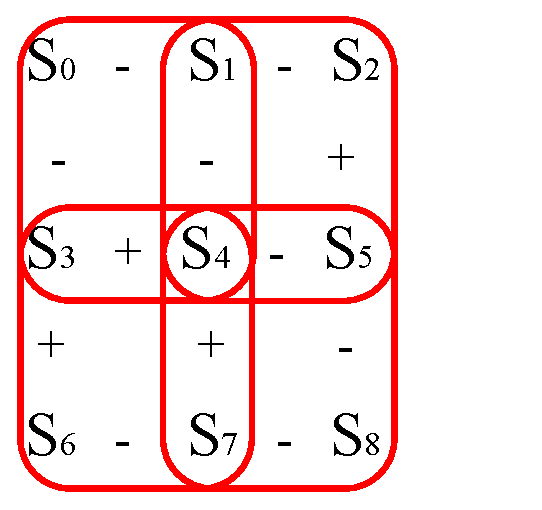
\includegraphics{3x3.eps}}
	\caption{Решётка 3x3}
	\label{fig:3x3}
\end{figure}

В кластере состоящем из четырёх фрустрированных подрешёток 2x2 \ref{fig:3x3} все фрустрированные пары расположены на пересечениях.

\begin{table}[h]
	\centering
	\begin{tabular}{|c|c|}
		\hline
		E   &   Фрустрированная пара \\
		\hline
		-8   &  $S_3=1$, $S_4=-1$\\
		&    $S_4=-1$, $S_5=-1$ \\
		\hline
		-8   &  $S_1=1$, $S_4=1$\\
		&    $S_4=1$, $S_7=-1$ \\
		\hline
		-8   &  $S_3=-1$, $S_4=1$\\
			&    $S_4=1$, $S_5=1$ \\
		\hline
		-8   &  $S_1=-1$, $S_4=-1$\\
			&    $S_4=-1$, $S_7=1$ \\
		\hline
	\end{tabular}
	\caption{Основные состояния решётки 3x3}
	\label{tab:gs_3x3}
\end{table} 

\begin{figure}[h]
	\centering
	\resizebox{150px}{150px}{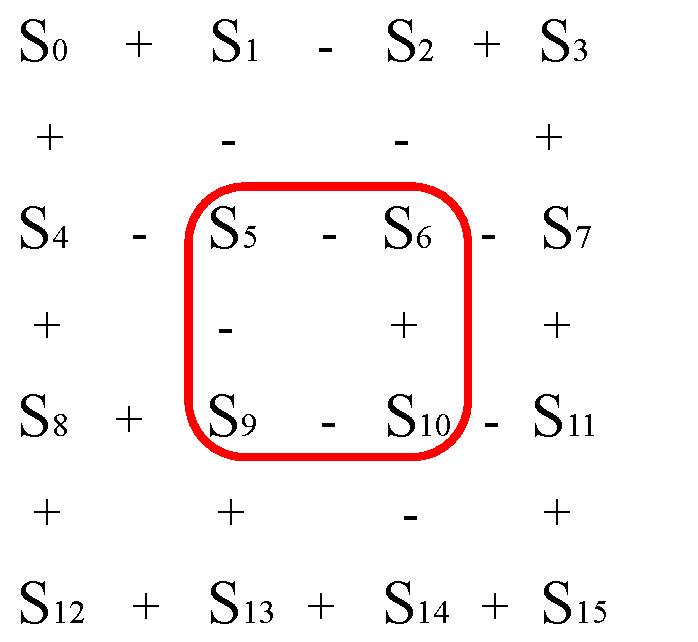
\includegraphics{4x4.eps}}
	\caption{Решётка 4x4}
	\label{fig:4x4}
\end{figure}

Если фрустрированная решётка 2x2 не образует кластер и не имеет пересечений с решётками подобного типа, но при этом вс же имеет пересечения с другими подрешётками как на  рисунке \ref{fig:4x4}, то какую бы пару в выделенной подрешётке мы не посчитали фрустрированной она будет возбуждать соседнюю подрешётку и в ней будет появляться вторая фрустрация причём таким, образом чтобы не возбуждать другие подрешётки 2x2. 

\begin{table}[h]
	\centering
	\begin{tabular}{|c|c|}
		\hline
		E   &   Фрустрированная пара \\
		\hline
		-20   &  $S_5=1$, $S_6=1$\\
		&    $S_1=-1$, $S_2=-1$ \\
		\hline
		-20   &  $S_5=1$, $S_9=1$\\
		&    $S_4=-1$, $S_8=1$ \\
		\hline
		-20   &  $S_6=1$, $S_{10}=-1$\\
		&    $S_7=-1$, $S_{11}=1$ \\
		\hline
		-20   &  $S_9=1$, $S_{10}=1$\\
		&    $S_{13}=1$, $S_{14}=-1$ \\
		\hline
		-20   &  $S_5=-1$, $S_6=-1$\\
		&    $S_1=1$, $S_2=1$ \\
		\hline
		-20   &  $S_5=-1$, $S_9=-1$\\
		&    $S_4=1$, $S_8=-1$ \\
		\hline
		-20   &  $S_6=-1$, $S_{10}=1$\\
		&    $S_7=1$, $S_{11}=-1$ \\
		\hline
		-20   &  $S_9=-1$, $S_{10}=-1$\\
		&    $S_{13}=-1$, $S_{14}=1$ \\
		\hline
	\end{tabular}
	\caption{Основные состояния решётки 4x4}
	\label{tab:gs_4x4}
\end{table}

Основные состояния данной решётки полученные полным перебором \ref{tab:gs_4x4} подтверждают что одна фрустрированная пара находится в выделенной области, а вторая в соседней подрешётки так, чтобы не пересекаться с другими подрешётками то есть с краю.

\begin{figure}[h]
	\centering
	\resizebox{310px}{220px}{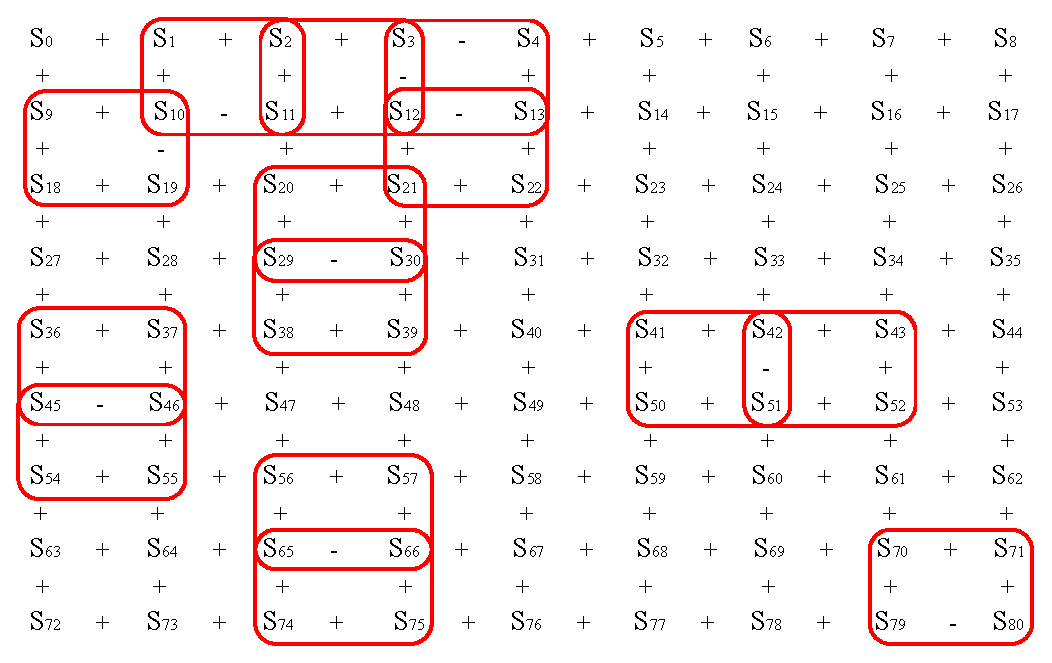
\includegraphics{9x9.eps}}
	\caption{Квадратная решётка из 81 спина}
	\label{fig:label_9x9}
\end{figure}



Определить основные состояния можно и на решётках больших размеров \ref{fig:label_9x9}, применяя все те же самые рассуждения. Энергия основного состояния, его кратность вырождения и спиновый избыток также совпадает с решением исчерпывающим перебором.

\begin{figure}[h]
	\centering
	\resizebox{310px}{220px}{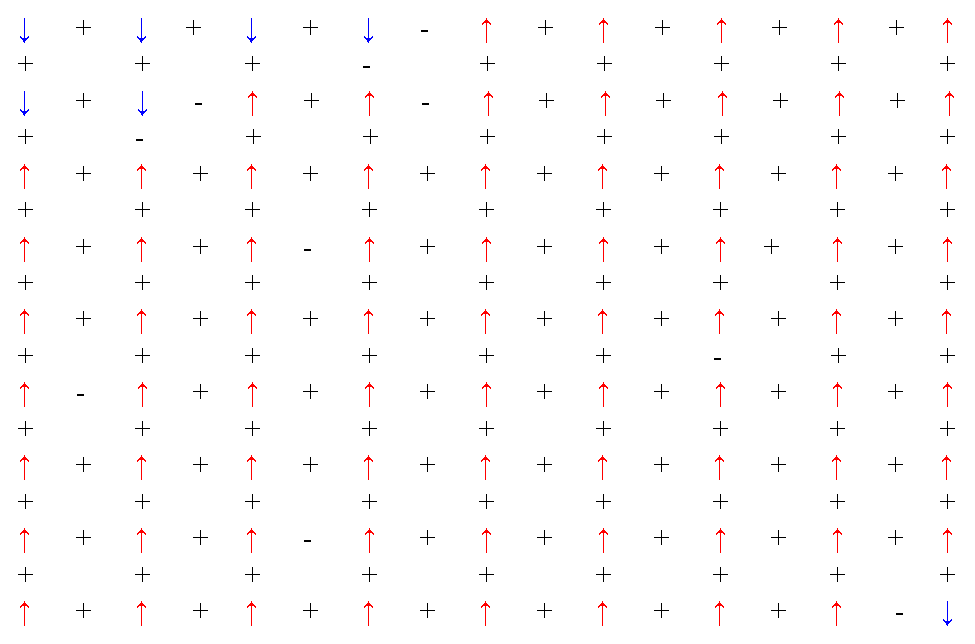
\includegraphics{9x9_gs_1.eps}}
	\caption{Одно из основных состояний решётки \eqref{fig:label_9x9}}
	\label{fig:label_9x9_gs_1}
\end{figure}


\section{Заключение}

С помощью разработанных программ ЭВМ на основании авторского подхода, а также с помощью известных методов возможно проведение исследований основных состояний фрустрированных спиновых моделей на решетках, расчет фазовой диаграммы в отсутствии температуры, исследование возбуждений и макроскопического вырождения основного состояния в зависимости от поля, поведения спинового избытка, конфигураций основного состояния во внешнем магнитном поле для развития физики конденсированного состояния.



\section{Благодарности}

 

\bibliography{mybibfile}


\end{document}